\documentclass[11pt]{book}

\usepackage[width=7.0in, height=9.0in, top=1.0in, papersize={8.5in,11in}]{geometry}
\usepackage[pdftex]{graphicx}
%\usepackage{datetime}
\usepackage{anyfontsize}
\usepackage{t1enc}
\usepackage{verbatim}
\usepackage{algorithm}
\usepackage{algorithmic}
\usepackage{framed}
\usepackage{pdfpages}
\usepackage{listings}
\lstset{language=C}

\lstset{language=python,frame=ltrb,framesep=5pt,basicstyle=\normalsize,
 keywordstyle=\ttfamily\color{DarkRed},
%morecomment=[n][\textbf]{In\ [}{]\:},
%morecomment=[n][\textbf]{Out\ [}{]\:},
morecomment=[s][\color{blue}]{In\ [}{]\:},
morecomment=[s][\color{red}]{Out[}{]\:},
identifierstyle=\ttfamily\color{DarkBlue}\bfseries,
commentstyle=\color{DarkGreen},
stringstyle=\ttfamily,
showstringspaces=false,tabsize = 3}


\lstdefinelanguage{shell} {
commentstyle = \color{black},
keywordstyle = \color{black},
stringstyle = \color{black},
identifierstyle = \color{black},
morecomment=[s][\color{blue}]{In\ [}{]\:},
morecomment=[s][\color{red}]{Out[}{]\:},
 }

\pagestyle{empty}

\usepackage{helvet}
\renewcommand{\familydefault}{\sfdefault}

\begin{document}

{\fontsize{16}{16}\selectfont Sprint Report \#2}

\section*{Team Overview}
\hrulefill
\subsection*{Members}
Mackenzie Smith, Alex Nienhueser

\subsection*{Project Title}
Dahl Virtual Museum Tour

\subsection*{Company}
Dahl Arts Center


\section*{Sprint Report}
\hrulefill
\subsection*{Work Accomplished}
\begin{itemize}
\item Free movement prototype
\item On-Rails prototype
\item Oculus integration in Unreal

\end{itemize}
\subsection*{Work Left}
\begin{itemize}
\item User documentation
\item VR integration with gallery room
\item Finalize gallery room with textures and art pieces
\item Guided tour system with narration
\item Free-moving tour
\item Research
\end{itemize}

\section*{Research}
The research done in the project so far has been focused on movement methods.  Both on-rails and free movement have been developed, which will be discussed later.  After the client presentation the idea of crowd sourcing the movement testing looks like a really good idea, which will be included in a future sprint, most likely in the next sprint.  The things that we will be focusing our research on will be movement speed, as well as movement controls to hopefully find a method of movement that results in the least amount of simulation sickness.

\section*{Client Interactions}
Over the course of this sprint, we had two meetings with Dr. Adkins, the first being a demo of the Oculus and the second was towards the end which was about starting sprint 3.  

During the first meeting we asked him his thoughts about his experience using the Oculus. The first demo was stationary, with no movement other than the head motion; he thought it was "super cool" and that he could not wait to see the final product.  The other demo we showed was a free movement demo that used the WASD keys for movement and the mouse for direction.  This is not the method we will be using in our project, but we wanted to gauge his thoughts on his experience in particular with simulation sickness.  Surprisingly he said he did not feel very sick but said he could definitely see how it could become a problem.

During our second meeting, we discussed what will be done during sprint 3, mainly the on-rails tour finalization which included the order in which the paintings should appear.  Other topics included getting the text descriptions prepared for the beginning of sprint 4 which is where they will be implemented, and a follow-up discussion about our client presentation.


\section*{Code Samples}
The movement Blueprints developed this sprint were mostly made by Alex, Mack helped a little bit in suggesting different ways to go about it, however Alex did the actual coding.  The following blueprint samples are from the two different movement methods that will be used in our project.  The on-rails blueprint use an array of coordinates called Waypoints.  This array will be navigated through by incrementing or decrementing causing the user to move to that point in a slow motion.

\begin{figure}
\caption{The blueprint used for free movement.  Movement values are changed in Unreal settings based on user feedback.}
\centering
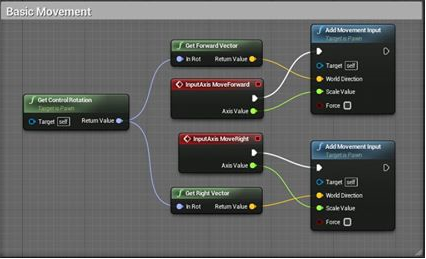
\includegraphics[scale=1.0]{basicMovement.png}
\end{figure}

\begin{figure}
\caption{First half of the on-rails blueprint}
\centering
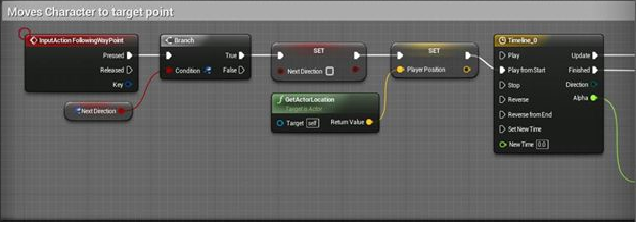
\includegraphics[scale=1.0]{moveToPoint.png}
\end{figure}

\begin{figure}
\caption{Second half of the on-rails blueprint}
\centering
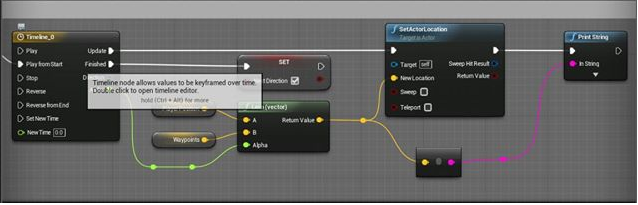
\includegraphics[scale=1.0]{moveToPoint2.png}
\end{figure}



\end{document}